\documentclass[11pt]{article} 
\usepackage[english]{babel}
\usepackage[utf8]{inputenc}
\usepackage[margin=0.5in]{geometry}
\usepackage{amsmath}
\usepackage{amsthm}
\usepackage{amsfonts}
\usepackage{amssymb}
\usepackage[usenames,dvipsnames]{xcolor}
\usepackage{graphicx}
\usepackage[siunitx]{circuitikz}
\usepackage{tikz}
\usepackage[colorinlistoftodos, color=orange!50]{todonotes}
\usepackage{hyperref}
\usepackage[numbers, square]{natbib}
\usepackage{fancybox}
\usepackage{epsfig}
\usepackage{soul}
\usepackage[framemethod=tikz]{mdframed}
\usepackage[shortlabels]{enumitem}
\usepackage[version=4]{mhchem}
\usepackage{multicol}
 
\usepackage{mathtools}
\usepackage{comment}
\usepackage{enumitem}
\usepackage[utf8]{inputenc}
\usepackage[linesnumbered,ruled,vlined]{algorithm2e}
\usepackage{listings}
\usepackage{color}
\usepackage[numbers]{natbib}
\usepackage{subfiles}
\usepackage{tkz-berge}


\newtheorem{prop}{Proposition}[section]
\newtheorem{thm}{Theorem}[section]
\newtheorem{lemma}{Lemma}[section]
\newtheorem{cor}{Corollary}[prop]

\theoremstyle{definition}
\newtheorem{definition}{Definition}

\theoremstyle{definition}
\newtheorem{required}{Problem}

\theoremstyle{definition}
\newtheorem{ex}{Example}


\setlength{\marginparwidth}{3.4cm}
%#########################################################

%To use symbols for footnotes
\renewcommand*{\thefootnote}{\fnsymbol{footnote}}
%To change footnotes back to numbers uncomment the following line
%\renewcommand*{\thefootnote}{\arabic{footnote}}

% Enable this command to adjust line spacing for inline math equations.
% \everymath{\displaystyle}

% _______ _____ _______ _      ______ 
%|__   __|_   _|__   __| |    |  ____|
%   | |    | |    | |  | |    | |__   
%   | |    | |    | |  | |    |  __|  
%   | |   _| |_   | |  | |____| |____ 
%   |_|  |_____|  |_|  |______|______|
%%%%%%%%%%%%%%%%%%%%%%%%%%%%%%%%%%%%%%%

\title{
\normalfont \normalsize 
\textsc{CSCI 3104 Spring 2022 \\ 
Instructors: Profs. Chen and Layer} \\
[10pt] 
\rule{\linewidth}{0.5pt} \\[6pt] 
\huge Quiz 23 - DP: Bellman-Ford algorithm \\
\rule{\linewidth}{2pt}  \\[10pt]
}
%\author{Your Name}
\date{}

\begin{document}
\definecolor {processblue}{cmyk}{0.96,0,0,0}
\definecolor{processred}{rgb}{200, 0, 0}
\definecolor{processgreen}{rgb}{0, 255, 0}
\DeclareGraphicsExtensions{.png}
\DeclareGraphicsExtensions{.gif}
\DeclareGraphicsExtensions{.jpg}

\maketitle


%%%%%%%%%%%%%%%%%%%%%%%%%
%%%%%%%%%%%%%%%%%%%%%%%%%%
%%%%%%%%%%FILL IN YOUR NAME%%%%%%%
%%%%%%%%%%AND STUDENT ID%%%%%%%%
%%%%%%%%%%%%%%%%%%%%%%%%%%
\noindent
Due Date \dotfill April 8 \\
Name \dotfill \textbf{Julia Troni} \\
Student ID \dotfill \textbf{109280095} \\

\tableofcontents

\section{Instructions}
 \begin{itemize}
	\item The solutions \textbf{should be typed}, using proper mathematical notation. We cannot accept hand-written solutions. \href{http://ece.uprm.edu/~caceros/latex/introduction.pdf}{Here's a short intro to \LaTeX.}
	\item You should submit your work through the \textbf{class Canvas page} only. Please submit one PDF file, compiled using this \LaTeX \ template.
	\item You may not need a full page for your solutions; pagebreaks are there to help Gradescope automatically find where each problem is. Even if you do not attempt every problem, please submit this document with no fewer pages than the blank template (or Gradescope has issues with it).

	\item You \textbf{may not collaborate with other students}. \textbf{Copying from any source is an Honor Code violation. Furthermore, all submissions must be in your own words and reflect your understanding of the material.} If there is any confusion about this policy, it is your responsibility to clarify before the due date. 

	\item Posting to \textbf{any} service including, but not limited to Chegg, Discord, Reddit, StackExchange, etc., for help on an assignment is a violation of the Honor Code.

\end{itemize}

\newpage
\section{Standard 23 - DP: Bellman-Ford algorithm}

\begin{required}

Consider the weighted directed graph $G(V, E, w)$ pictured below. Work through the Bellman-Ford algorithm with the destination vertex $C$. 
\begin{itemize}
\item Clearly specify the cost $d(v)$ of the current  best path from each node $v\in V$ to $C$ as well as the corresponding successor node  at each iteration/pass. You may want to make a table to store the costs and successors.

\item Give the shortest path tree, i.e., the union of all the shortest paths to $C$ from all other vertices. For your convenience, you may want to modify the ``latex code" for the given graph to draw the shortest path tree.

\end{itemize}

\definecolor {processblue}{cmyk}{0.96,0,0,0}
\begin{center}
	\begin {tikzpicture}[-latex ,auto ,node distance =1.5cm and 2cm ,on grid ,
	semithick ,
	state/.style ={ circle ,top color =white , bottom color = processblue!20 ,
	draw,processblue , text=blue , minimum width =0.5 cm}, scale=0.5]

	\node[state] (A) {$A$};
	\node[state] (B) [above right = of A] {$B$};
	\node[state] (C) [below right = of A] {$C$};
	\node[state] (E) [below right = of B] {$E$};
	\node[state] (D) [above right = of E] {$D$};
		
	
	\path (A) edge node[above] {$5$} (B);
	\path (A) edge node[above] {$10$} (C);
	\path (B) edge node[above] {$1$} (E);
	\path (D) edge node[above] {$1$} (B);
	\path (A) edge node[above] {$1$} (E);
	\path (D) edge node[above] {$3$} (E);	
	\path (E) edge node[above] {$2$} (C);
	
	\end{tikzpicture}  
\end{center}




\begin{proof}[Answer]
%Your answer here
Apply Bellman-Ford to the graph: \\
Let $c(u,v)$ denote cost of the edge from vertex u to vertex v. Let $D(v)$ denote the cost of the current path from vertex v to the destination vertex C. 
\begin{enumerate}
\item 1st iteration: begin by examining source vertex C incoming edges. 
	\begin{itemize}
	\item Poll edge (A,C): $D(A)=\infty > D(C)+c(A,C)=0+10$ so set $D(A)=10$ and $successor[A]=C$
	\item Poll edge (E,C): $D(E)=\infty > D(C)+c(E,C)=0+2$ so set $D(E)=2$ and $successor[E]=C$
	\end{itemize}
\item 2nd iteration:examine the incoming edges for each of the updated vertices, which were A, C 
	\begin{itemize}
	\item Poll edge (A,E): $D(A)=10 > D(E)+c(A,E)=2+1=3$ so set $D(A)=2$ and $successor[A]=E$
	\item Poll edge (D,E): $D(D)=\infty < D(E)+c(D,E)=2+3$ so set $D(D)=5$ and $successor[D]=E$
	\item Poll edge (B,E): $D(B)=\infty> D(E)+c(D,E)=2+1=3$ so set $D(B)=3$ and $successor[B]=E$
	\end{itemize}
\item 3rd iteration:examine the incoming edges for each of the updated vertices, which were A,D,B 
	\begin{itemize}
	\item Poll edge (A,B): $D(A)=3< D(B)+c(A,B)=3+5=8$ so no change
	\item Poll edge (D,B): $D(D)=5 > D(B)+c(D,B)=3+1=4$ so set $D(D)=4$ and $successor[D]=B$
	\end{itemize}
\item 4th iteration:no updates made
\end{enumerate}
At the end of the algorithm the paths are the following\\
\begin{itemize}
\item A-E-C with cost of 3
\item B-E-C with cost 3
\item E-C with cost 2
\item D-B-E-C with cost 4
\end{itemize}
See the shortest path tree below \\
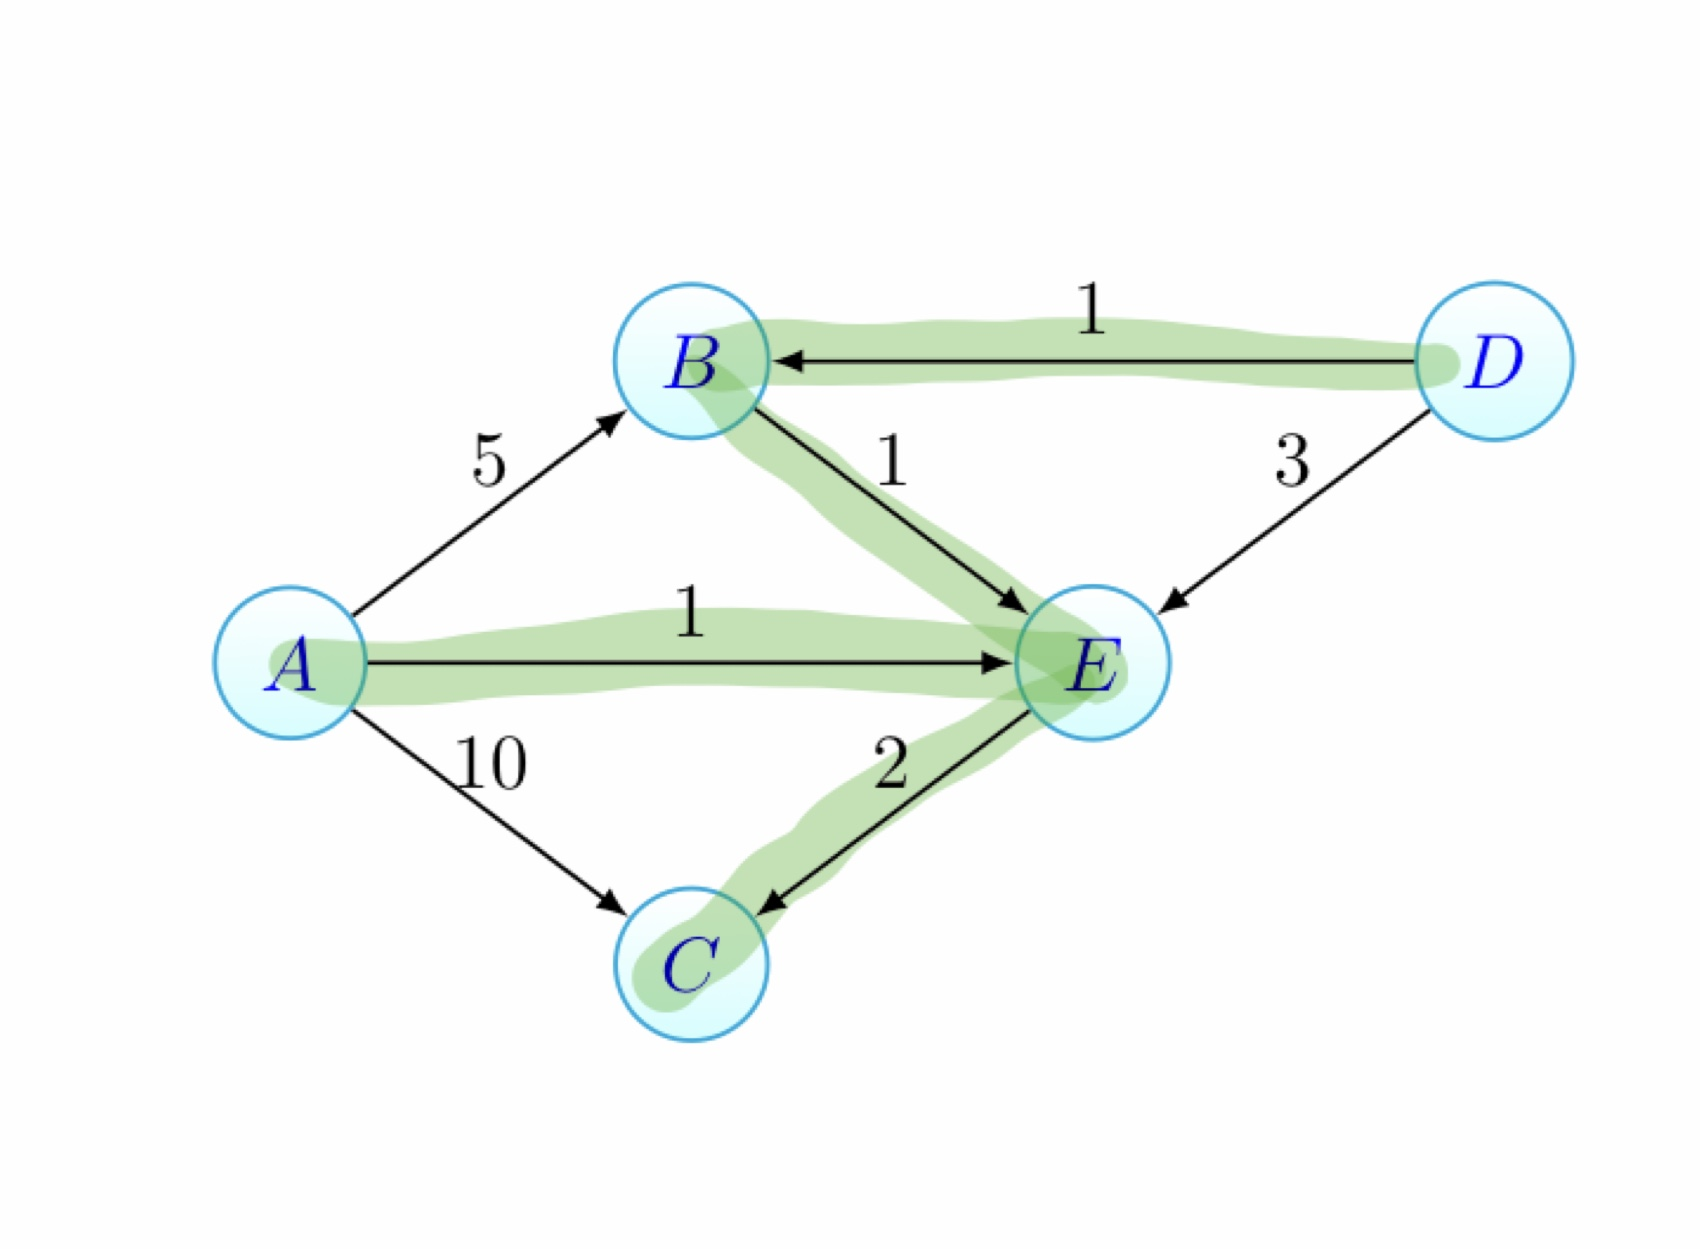
\includegraphics[width=0.8\textwidth]{q23}

\end{proof}


\end{required}

%%%%%%%%%%%%%%%%%%%%%%%%%%%%%%%%%%%%%%%%%%%%%%%%%%
\end{document} % NOTHING AFTER THIS LINE IS PART OF THE DOCUMENT



